\documentclass[11pt,a4paper,sans]{moderncv} % Font sizes: 10, 11, or 12; paper sizes: a4paper, letterpaper, a5paper, legalpaper, executivepaper or landscape; font families: sans or roman

\moderncvstyle{banking} % CV theme - options include: 'casual' (default), 'classic', 'oldstyle' and 'banking'
\moderncvcolor{grey} % CV color - options include: 'blue' (default), 'orange', 'green', 'red', 'purple', 'grey' and 'black'

\usepackage[scale=0.75]{geometry} % Reduce document margins
%\setlength{\hintscolumnwidth}{3cm} % Uncomment to change the width of the dates column
%\setlength{\makecvtitlenamewidth}{10cm} % For the 'classic' style, uncomment to adjust the width of the space allocated to your name

%\usepackage{hyperref}
\usepackage{graphicx}

\usepackage{subcaption}
\usepackage{tikz}
\usetikzlibrary{arrows,automata,positioning}

\title{Research Plan}

\firstname {Sreejith}
\familyname {A V}

\begin{document}
\makecvtitle % Print the CV title

\section{Introduction}
My research lies at the intersection of theoretical computer science and practical applications, with a focus on logic, automata theory, and their integration into fields like formal verification and recently machine learning. I completed my Ph.D. under Prof. Kamal Lodaya at the Institute of Mathematical Sciences, Chennai, and subsequently pursued postdoctoral research at institutions such as IRIF, France, and the University of Warsaw, Poland. Currently, I am an Associate Professor at IIT Goa. \\

My initial work concentrated on the theoretical foundations of logic and automata. Over time, I expanded into applied research, leveraging formal methods to address challenges in verification, and machine learning. This document outlines my contributions, current work, and future directions.

\section{Descriptive Complexity: Ph.D.}
Logic provides a precise framework to express mathematical properties unambiguously. It plays a vital role in areas like descriptive complexity~\cite{immerman_book}, and set theory~\cite{ject_setTheory}.
%While Hilbert's program sought to axiomatize mathematics, Gödel's incompleteness theorem underscored the limits of formal systems \cite{godel_incompleteness}. Yet, l
Logic has driven advances among other things in formal verification, database, and artificial intelligence~\cite{vardi_logicEffectiveness}.

\subsection{Contributions}
My Ph.D. thesis \cite{sav_thesis} introduced modulo counting operators, thereby enhancing the expressiveness of logics. Key contributions include:
\begin{enumerate}
 \item Extending Linear temporal logic (\textsf{LTL}) with modulo counting operators, enhancing its expressiveness while retaining PSPACE complexity for model checking~\cite{my_ltlmod,my_ltlsuccinct}.
 \item Resolving an \emph{open problem} in circuit complexity by showing that certain regular languages are not definable in first-order logic with addition and modulo counting operators~\cite{my_foplus}. It connects logic and semigroup theory to show strict hierarchies in certain highly uniform circuit classes.
\end{enumerate}

\subsection{Awards and Recognition}
\begin{itemize}
    \item \textbf{ACM India Honorable Mention (2014):} Ph.D. thesis titled \emph{Regular Quantifiers in Logics}.
\end{itemize}

\section{Countable Words: Postdoctoral and IIT Goa}
This work is at the meeting point of two important branches of language theory: on the one hand the extension of the finite word language theories~\cite{Kleene56,RabinScott59}, in particular infinite words~\cite{Buchi62} or infinite trees~\cite{Rabin69}, as initiated by Büchi, and on the other hand the characterization of classes of languages, in particular logics, as initiated by Schützenberger \cite{Schutzenberger65}.
%Language theory originated with finite words and extended to infinite words~\cite{Buchi62} and trees~\cite{Rabin69}, leading to MSO decidability for these structures.
In our case, we study countable words, the largest extension that is known to have a theory of recognizability.

\subsection{Contributions}
Our work provided the first algebraic characterizations of intermediate logics over countable words:
\begin{itemize}
    \item Developed characterizations (algebraic / regular expression) for logics such as first-order logic (\textsf{FO}), \textsf{FO}$^2$, \textsf{FO} with cuts, weak \textsf{MSO}, and scattered \textsf{FO}, yielding decidability results~\cite{icalp15,ms16}.
    \item Established decomposition theorems for algebraic structures in this context~\cite{lics19,jcss23}.
    \item Demonstrated that certain logics, such as \textsf{FO} with cuts and weak \textsf{MSO}, cannot be decomposed using a finite set~\cite{fct21}.
\end{itemize}
These results provide tools for comparing expressiveness among logics.

\subsection{Achievements}
\begin{itemize}
    \item \textbf{Supervision:} Informally co-superviced Saptarshi Sarkar (Ph.D. under Bharat Adsul, IIT Bombay).
\end{itemize}


\section{One-Counter Automata: IIT Goa}
Finite automata models complex systems, from computational processes \cite{vardi95} to biological phenomena \cite{Barto75}.
Deterministic one-counter automata (DOCA) extend deterministic finite automata with an integer counter. It captures behavior of infinite-state systems. See Figure 1.

\subsection{Contributions}
We addressed two key problems:
\begin{itemize}
    \item \textbf{Equivalence of weighted DOCA:} We showed decidability for a large subclass using novel reachability techniques, placing the problem in P \cite{fsttcs23,icla25}. The equivalence problem for the full class is an important open problem in the area.
    \item \textbf{Active learning algorithms for DOCAs:}
    \begin{itemize}
    \item Developed SAT-based algorithm~\cite{learning24} that is better than state of the art algorithm \cite{gaetan}.
    \item Developed the first polynomial-time algorithm, significantly advancing the state-of-the-art (unpublished). This work will enable faster and more efficient active learning of DOCAs.
    \end{itemize}
\end{itemize}

\subsection{Achievements}
\begin{itemize}
    \item \textbf{Funding:} SERB research grant for \emph{Probabilistic Pushdown Automata} (2021--2024).
    \item \textbf{Supervision:} Prince Mathew (Ph.D. student), expected to submit thesis by Dec 2024.
\end{itemize}
\begin{minipage}{\textwidth}
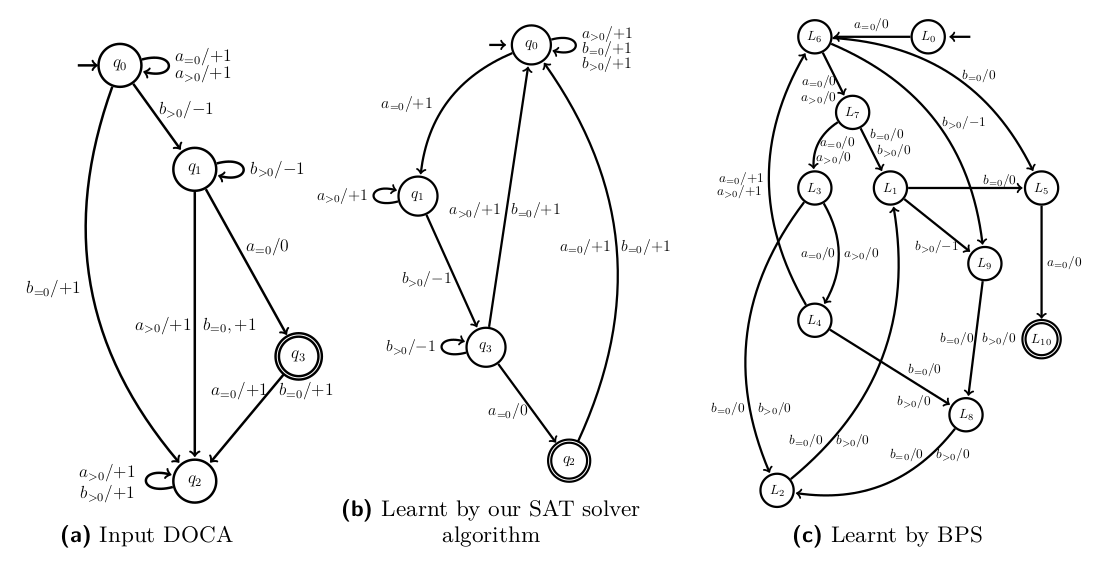
\includegraphics[width=0.85\textwidth]{doca.png} \\
\textbf{Figure 1} The input DOCA recognizes the language $\{a^nb^na ~|~ n > 0\}$.
\end{minipage}

%\clearpage

\section{Water Research Using Geostationary Data}
In collaboration with environmental scientists, we developed methods to estimate river water discharge (see Figure 2.) using geospatial data (along with in-situ measurements) \cite{esd21}. Ongoing work focuses on soil moisture estimation, contributing to water resource management.

\subsection{Achievements}
\textbf{Funding:} Ministry of Earth Science (MoES) sanctioned project \emph{Remote sensing based method
for detecting water discharge in the Ganga and Brahmaputra rivers}.

\begin{minipage}{\textwidth}
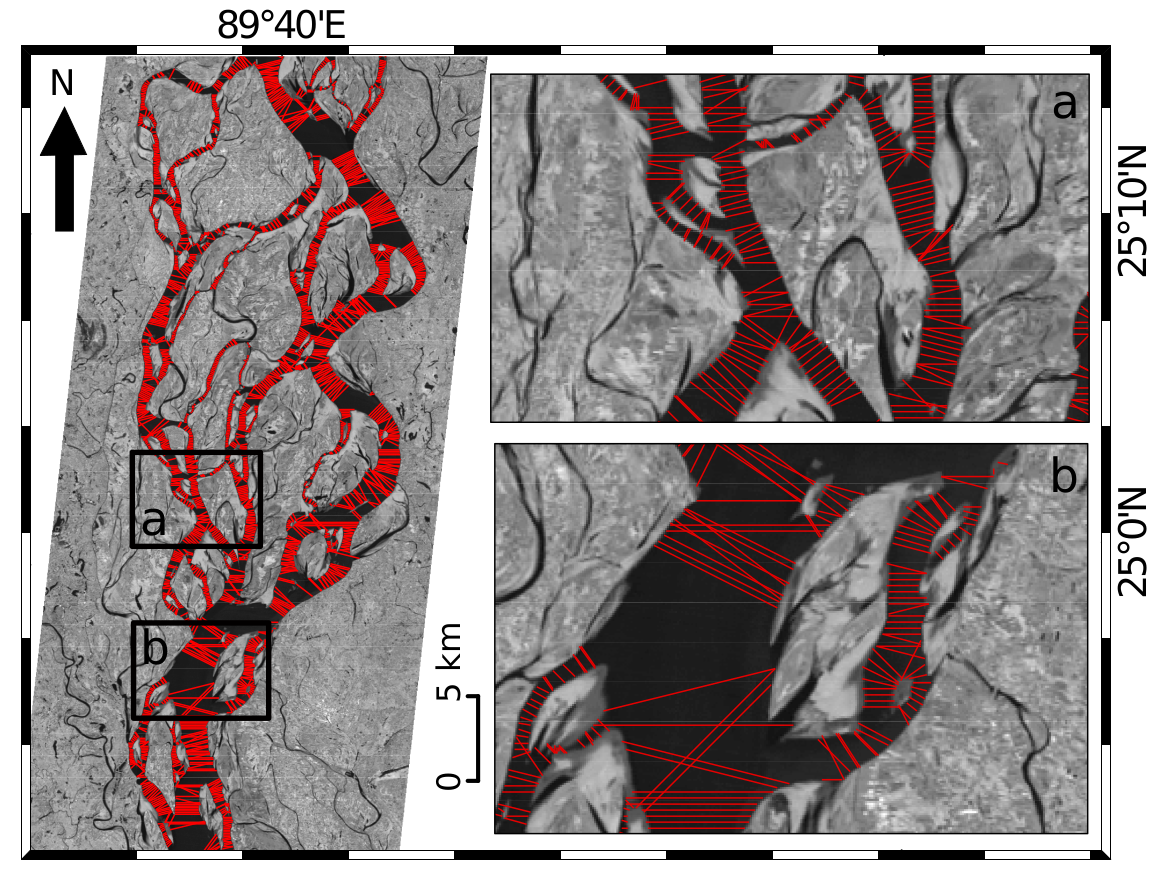
\includegraphics[width=0.6\textwidth]{river-width.png} \\
  \textbf{Figure 2} River width estimation.
\end{minipage}

\section{Formal Methods in Machine Learning: Future Directions}
Adaptive control systems in safety-critical applications (e.g., autonomous vehicles, robotics) require rigorous verification. Verifying their safety poses significant challenges when these controllers use machine learning algorithms for their decision making. In safety critical systems, it is important
to ensure that the overall safety of the controller is not compromised. My research proposes formal verification techniques using abstraction and SAT/SMT solvers to ensure safety in such systems.

\subsection{Future directions}
\begin{itemize}
 \item Developing scalable verification techniques for machine learning models.
 \item Developing verification techniques for control systems that use machine learning algorithms inside.
\end{itemize}

\subsection{Achievements}
\begin{itemize}
    \item \textbf{Funding:} Indo-French grant (CEFIPRA) for \emph{Formal Verification of Adaptive Control Algorithms}.
    \item \textbf{Visiting Faculty and Funding:} University of Bordeaux, contributing to research on \emph{Formal methods in machine learning}.
\end{itemize}


\section{Conclusion}
My research combines theoretical rigor with practical applications, advancing logic, automata theory, and their implications in formal verification. In the next decade, I aim to:
\begin{itemize}
    \item Continue the foundational work in automata theory and logic.
    \item Design and develop algorithms and tools for formal verification of machine learning systems.
    \item Expand interdisciplinary collaborations, applying theoretical methods to water research.
\end{itemize}


\bibliographystyle{alpha}
\bibliography{papers}

\end{document}
